\section{Resultados e discussões}
\subsection{Sistema massa-mola}
%Done: freq de oscilações
%Done: const elástica da mola
%Done: relação massa ~ freq
A partir dos dados extraídos do Tracker, resumidos nas \cref{molaG,molaP,molaG2m}, é notável observar o comportamento senoidal de todos os sistemas. É possível estimar a frequência do sistema massa-mola pela observação gráfica. Em \cref{molaG} a observação indica aproximadamente 1 oscilação por segundo. Enquanto em \cref{molaP} obtêm-se pouco mais de uma oscilação por segundo. E, em \cref{molaG2m} pouco menos de 1 oscilação por segundo.

\begin{figure}[h]
    \centering
    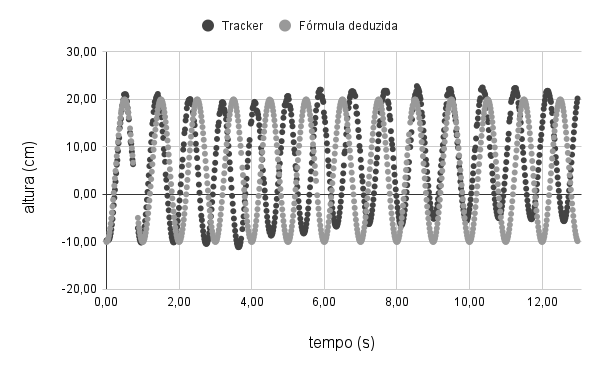
\includegraphics[width=.5\linewidth]{fig/molaG}
    \caption{Para mola grande com massa de \qty{100}{g}, gráfico de dispersão dos dados obtidos no Tracker em comparação aos valores nos mesmos instantes de tempo com a função horária deduzida}\label{molaG}
\end{figure}

\begin{figure}[h]
    \centering
    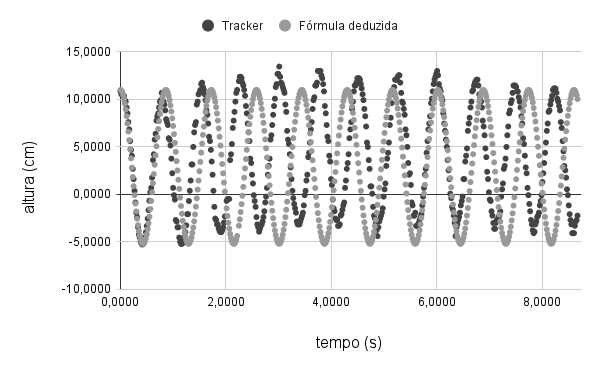
\includegraphics[width=.5\linewidth]{fig/molaP}
    \caption{Para mola pequena com massa de \qty{100}{g}, gráfico de dispersão dos dados obtidos no Tracker em comparação aos valores nos mesmos instantes de tempo com a função horária deduzida}\label{molaP}
\end{figure}
 
No entanto, podemos também nos aproveitar do comportamento dos sistemas e obter uma equação para descrever cada um dos sistemas a partir da função horária da posição da massa considerando que tenha comportamento de um oscilador harmônico simples: 

\begin{align*}
    x(t) = A\cos(\omega t + \psi) + x_0
\end{align*}

Para o sistema com a mola maior e a massa de \qty{100}{\gram}, considerando os primeiros períodos, obtemos que os pontos de máximo e mínimo são: \(x(0) = \qty{-10}{cm}\), \(x(0,50) = \qty{20}{cm}\). Então, podemos extrair a função horária:

\begin{align*}
    x_{Gm}(t) = A\cos(\omega t + \psi) + x_{Gm0}\\
    x_{Gm}(0) = A + x_{Gm0} = \qty{20}{cm} \\
    x_{Gm}(1) = -A + x_{Gm0} = \qty{-10}{cm} \\
    \implies x_{Gm0} = \qty{5}{cm}\\
    \implies A = \qty{20}{cm} - \qty{5}{cm} = \qty{15}{cm}\\
    \text{Além de que:}\\
    x_{Gm}(0) \text{é mínimo} \implies \cos(\psi) = -1\\
    \implies \psi = \pi\\
    x_{Gm}(0,50) \text{é máximo} \implies \cos(0,5\omega + \pi) = 1\\
    \implies \omega = 2 \pi\\
    \implies x_{Gm}(t) = 15\cos(2\pi t + \pi) + 5\\
    \implies x_{Gm}(t) = -15\cos(2\pi t) + 5
\end{align*}

Esta é a fórmula deduzida para o sistema massa-mola apresentada em cinza na \cref{molaG}. É notável que a fórmula descreve bem o sistema nos períodos iniciais e começa a se comportar de maneira diferente ao longo de mais períodos. Esta divergência decorre de: (1) a dispersão de energia na forma de calor no sistema real, (2) a trepidação do sistema no eixo x, não oscilando perfeitamente na vertical, (3) a trepidação da câmera que registra o sistema, causando diferenças na altura absoluta da massa com relação a altura observada no software Tracker.

O mesmo processo pode ser utilizada para extrair a função horária da mola menor:

\begin{align*}
x_{pm}(t) = 8,1 \cos(\frac{\pi}{0,43}t) + 2,9
\end{align*}

    Que também apresenta divergências com relação aos dados extraídos do Tracker pela mesma justificativa que a mola maior, conforme observável na \cref{molaP}.
    Com as funções horárias é possível determinar a frequência dos osciladores:

\begin{align*}
    \nu = \frac{\omega}{2\pi}\\
    \nu_{pm} = \frac{\pi}{\num{0,43} \cdot 2\pi} = \num{1,16}\\ 
    \nu_{Gm} = \frac{2\pi}{2\pi} = 1
\end{align*}

Em que, \(\nu_{pm}\) é a frequência da mola pequena com massa de \qty{100}{g} e \(\nu_{Gm}\) é a mola grande com massa de \qty{100}{g}. Obtemos então, resultados compatíveis com a análise gráfica.

É possível determinar também a constante elástica das molas:
\begin{align*}
   k = \omega^2 \cdot m\\
   k_{pm} = {(\pi\qty{2}{\per\second})}^2 \cdot \qty{0.1}{\kilo\gram}\\
   k_{pm} = \qty{3,95}{\N\per\meter}\\
   k_{Gm} = {(\frac{\pi}{0.43}\qty{1}{\per\second})}^2 \cdot \qty{0.1}{\kg}\\
   k_{Gm} = \qty{5.34}{\N\per\meter} 
\end{align*}

A frequência de oscilação do sistema é determinada por \(\frac{\omega}{2 \pi}  = \nu\), com \(\omega^2 = \frac{k}{m}\), portanto, a frequência deve ser inversamente proporcional à raiz quadrada da massa. Podemos averiguar isso observando a frequência para o sistema com a massa grande com \qty{200}{\g}. A função derivada para esta mola é \(x_{G2m} = 8.84\cos(\frac{\pi}{0.66}t) -11.16\), é possível observar a comparação entre esta função e os dados extraídos do Tracker na \cref{molaG2m}. Desta função, podemos extrair \(\nu = \cfrac{\pi}{0.66 \cdot 2 \cdot \pi} = \qty{0.76}{\per\second}\). Como esperado, o valor obtido é menor que a frequência para a mesma mola com uma massa menor.   

\begin{figure}[h]
    \centering
    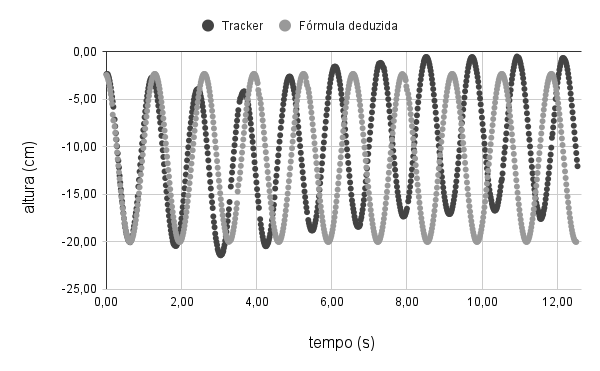
\includegraphics[width=.5\linewidth]{fig/molaG2m}
    \caption{Para mola grande com peso de \qty{200}{\g}, a figura apresenta os dados extraídos do software Tracker em comparação com os valores obtidos nos mesmos instantes de tempo para uma função horária deduzida para este oscilador}
    \label{molaG2m}
\end{figure}

           
\subsection{Ondas}
%TODO: como o ocorre formação de nós;
%TODO: qual a diff entre esfera que vibra e e as molas?

    
